\documentclass[12pt]{article}
\usepackage{color}
\usepackage[usenames,dvipsnames,svgnames,table]{xcolor}
\definecolor{dark-red}{rgb}{0.7,0.1,0.1} 
\definecolor{dark-blue}{rgb}{0,0,0.7} 
\usepackage[linkcolor=dark-red,
            colorlinks=true,
            urlcolor=dark-blue,
            pdfstartview={XYZ null null 1.00},
            pdfauthor={Gaurav Sood, gsood07@gmail.com},
            citecolor=dark-red,
            bookmarks=false,
            pdfborder={0 0 0},
            pdftitle={Fairly Random}]{hyperref}
            
\usepackage{amsfonts,amssymb,amsbsy,amsmath,amsxtra}

\usepackage[letterspace=1000]{microtype}
\usepackage{libertine}
\usepackage[T1]{fontenc}

\usepackage{indentfirst}
\usepackage{setspace} % To set line spacing
\usepackage{multirow}

\usepackage{verbatim}

\usepackage[multiple]{footmisc}
\usepackage{fancyvrb}

\usepackage{longtable}

\usepackage[margin=1in]{geometry}
\usepackage{graphicx}

\raggedright
\parindent=1.5em % <- or whatever indent you want

\usepackage{natbib}
\usepackage{url}
\begin{comment}

setwd(paste0(githubdir, "/cricket-stats/write_up/"))	
tools::texi2dvi("cricket.tex", pdf=TRUE, clean=TRUE)	
setwd(paste0(githubdir, "/cricket-stats/"))

\end{comment}

\begin{document}
\title{\vspace{-.5cm}\normalsize{Fairly Random: Impact of Winning the Toss on the Probability of Winning\footnote{You can find the scripts used to scrape the data, the final data set, and scripts used for analysis at: \href{https://github.com/dwillis/cricket-stats}{https://github.com/dwillis/cricket-stats}.}\vspace{.5cm}}}
\author{\normalsize{Gaurav Sood}\\\href{mailto:gsood07@gmail.com}{\small{gsood07@gmail.com}} \and \normalsize{Derek Willis}\\\href{mailto:dwillis@gmail.com}{\small{dwillis@gmail.com}}}
\date{\vspace{.5cm}\normalsize{\today}}
\maketitle
\doublespacing

In nearly all cricket matches, it is claimed that there is a clear advantage to bowling (batting) first. The advantage is pointed to by commentators, by the team captains in the pre-toss interview, and by the captain of the losing team in the post-match interview. And to wrest this said advantage, one merely needs to pick the side of the coin that will be left facing the sky after it is tossed. And while this method of granting advantage is fair on average, the system isn't fair in any one game. 

At first glance, the imbalance seems inevitable. After all, someone has to bat first. One can, however, devise a baseball like system where short innings are interspersed. If that violates the nature of the game too much, one can easily create pitches that don't deteriorate appreciably over the course of a game. Or, one can come up with an estimate of the advantage, and adjust scores accordingly, akin to an adjustment issued when matches are shortened due to rain.

None of this to say that there is actually an advantage in winning the toss, or that teams are able to successfully exploit any such advantage. For it may be impossible to predict well in advance the advantage of bowling or batting first. Or, it may be that teams squander the potential advantage by using bad heuristics to choose what they do.

To assess the net observed advantage of winning the toss, we leverage data from over 43,000 first-class men's cricket matches --- to our knowledge, largest ever dataset assembled for the question, and nearly 50--100 times larger than used in prominent previous attempts \citep[see,][]{dawson2009bat, de1998winning}. Using the data, we estimate the impact of winning the toss on the probability of winning a match. Unlike some other studies on the topic, e.g. \citet{dawson2009bat, Saad2015}, we do not condition on post coin-toss decisions to avoid post-treatment bias \citep[see][]{acharya2015}. We find that winning the toss grants a small but significant advantage, but that advantage varies considerably and systematically. 

\section*{Data}
Data are from 43,185 first-class men's cricket matches. It is a near census of the relevant population. We have data on all types of matches: domestic and international Twenty20s -- T20s and T20Is respectively, domestic and international one-dayers -- List A and One-Day Internationals (ODI) respectively, and domestic and international multi-day matches -- First Class (FC) and Tests respectively.\footnote{There is a rich variety of first-class matches. In English county cricket, first-class matches last four days. Some first class matches last just a day. Others two days. Yet others three days. And till a particular point in history, a test match lasted as long as it was needed to finish a game. We elide over such differences.} 

Of these matches, we do not have data on the toss for 2,807, or roughly 7\%, of the matches. The primary reason we don't have data on these matches is because the match was abandoned without play. We exclude data from these matches. 

In limited overs cricket, a minimum number of overs must be bowled to establish a result. In a one-day match, for instance, each side must bat at least 20 overs for a result to be declared. In 706 matches, or roughly 1.7\% of the remaining matches, not enough overs were bowled to get a result. We again exclude these matches from our analysis. This leaves us with 39,672 matches. We analyze these data.
 
\section*{Analyses and Results}

We assume that the outcome of a toss is random. Conditional on the outcome of a toss being random, the effect of winning a toss can be attributed to the toss itself. We begin by assessing the validity of the assumption. In particular, we assess whether teams win more tosses in their home country than outside. 

In cricket matches, three results are possible: a draw, a win, and a loss. We look at draws, a common outcome in matches in which overs aren't limited, later on. For now, we focus on winning and losing. We elide over differential number of draws across formats, estimating the difference in probability of winning and losing. 

A caveat about interpretation before we report the results. As we discuss in the introduction, we cannot estimate the actual advantage of winning a toss. We can only estimate the net observed advantage, which is the extent to which the teams capitalize on the potential advantage. 

The team that wins the toss wins the match 2.3\% more often than it loses it. This is a reasonable sized advantage in a competitive sport --- though likely much smaller than the number that most commentators carry in their heads. This advantage, however, is highly variable by format, by conditions, by whether or not a particular formula was used to adjust scores when it rains, and how much better the team that won the toss is vis-\`{a}-vis the competing team. Some of the variability is expected, but as we will see, expectations are often dashed. 

The conventional wisdom among the lay cricket followers is that toss grants the greatest advantage in multi-day affairs like tests and first class matches, followed by day long affairs, and Twenty20s respectively. And there is good dose of common sense behind the conventional wisdom. Pitches invariably deteriorate over multiple days and batting last in a test match is often challenging. The pitch deteriorates far less over the course of the day, or in case of Twenty20s -- a few hours. And indeed unlimited over matches provide the most consistent advantage -- the average advantage over FC and test matches is north of 2.2\% (see Figure~\ref{fig:type}). But the heftiest advantage is in domestic one-day matches (List A), approximately 4\%. The number for ODIs, however, is a bit puzzling -- there is a slight disadvantage to winning the toss. That can best be ascribed to choosing badly.      

\begin{figure}[htbp]
\centering
\caption{Percentage of Matches Won Minus Matches Lost After Winning the Toss by Type of Match}
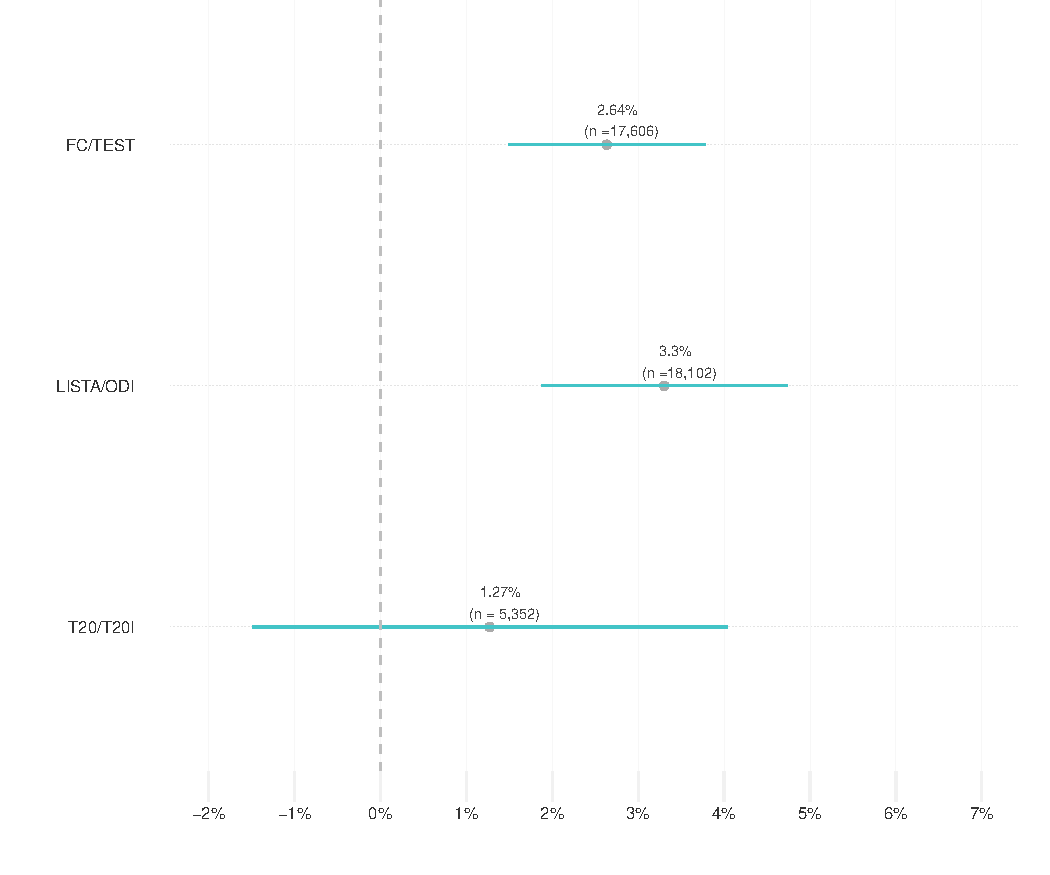
\includegraphics[scale=.85]{../figs/winbyType.pdf}
\label{fig:type}
\end{figure}

But type of matches cover only major source of variation and theorizing about the advantage granted by the toss. It is often claimed that the toss is more crucial in day and night matches. Due to dew -- it is thought to make bowling hard, and lower visibility of the white ball under lights -- it allegedly makes catching hard, it is thought that the team that fields second is disadvantaged. It turns out that the conventional wisdom is largely vindicated, except in the case of Twenty20 Internationals (see Figure ~\ref{fig:dn}). In each, domestic one-day and Twenty20 matches, and one-day internationals, the advantage of winning the toss is at least 3\%, and in case of one-day internationals, nearly 8\%.

\begin{figure}[htbp]
\centering
\caption{Percentage of Matches Won Minus Matches Lost After Winning the Toss By Day/Night}
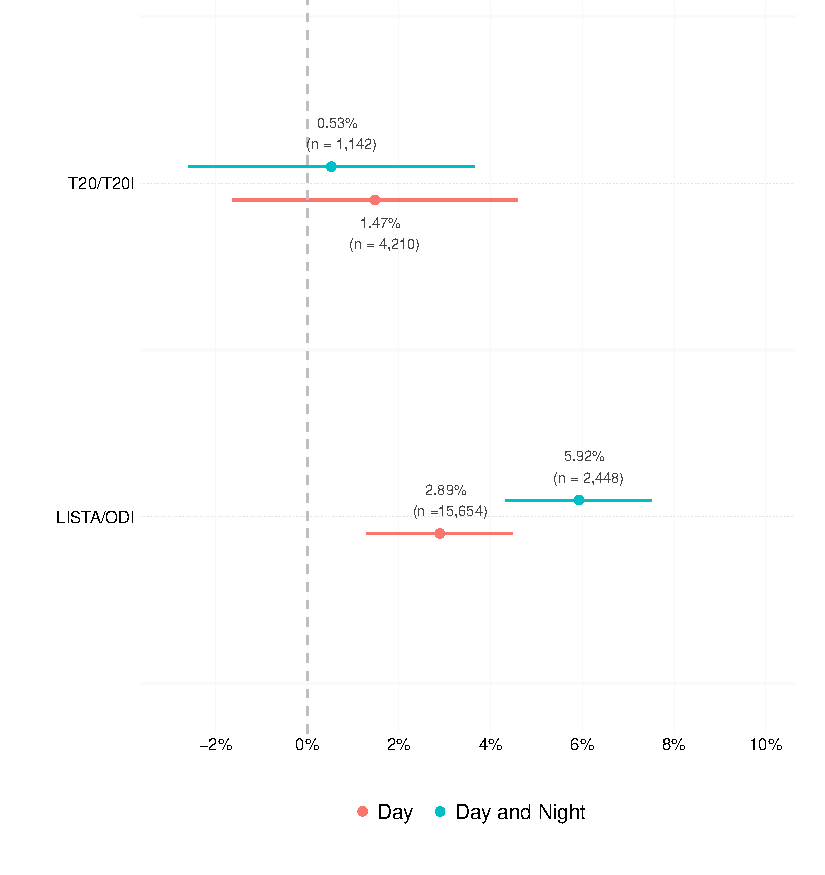
\includegraphics[scale=.85]{../figs/winbyDayNight.pdf}
\label{fig:dn}
\end{figure}

In limited over matches sometimes weather intervenes significantly after the match has already begun. After certain loss of time, the match is generally curtailed and the scores adjusted using a method invented by Duckworth and Lewis \citep[see][]{duckworth1998}. We can use the random nature of who wins the toss to see if winning percentages are strongly conditioned by matches that use Duckworth-Lewis and matches that don't. We find scant differences except in the case of international Twenty20s (see Figure ~\ref{fig:dl}).

\begin{figure}[htbp]
\centering
\caption{Percentage of Matches Won Minus Matches Lost After Winning the Toss by Duckworth-Lewis}
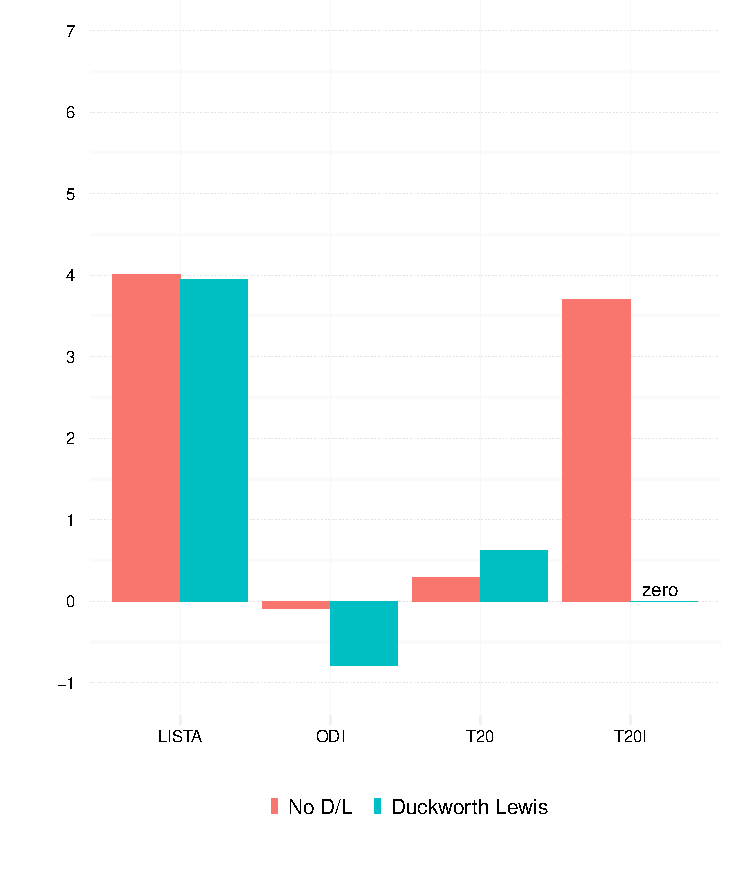
\includegraphics[scale=.85]{../figs/winbyDL.pdf}
\label{fig:dl}
\end{figure}

Lastly, winning a toss ought to matter the most when two closely matched teams are playing. What good would winning the toss do if you are matched with a team you have no chance beating. To study this, we collected ranking data. The ranking data are only available for international teams. And for reasons to do with convenience, we limited ourselves to collecting data on one-day internationals and tests between the earliest starting point and 2013. (These ranking data are updated monthly.) We measure how closely matched the teams are by simply subtracting the ranking points of team that lost the toss from the team that won it. The results are expected but new. As Figure ~\ref{fig:ranks}, there is a sharp curve around 0. When closely matched teams win, the winning ratio is strongly affected by who wins the toss.

\begin{figure}[htbp]
\centering
\caption{Percentage of Matches Won Minus Matches Lost After Winning the Toss by Difference in Ranks}
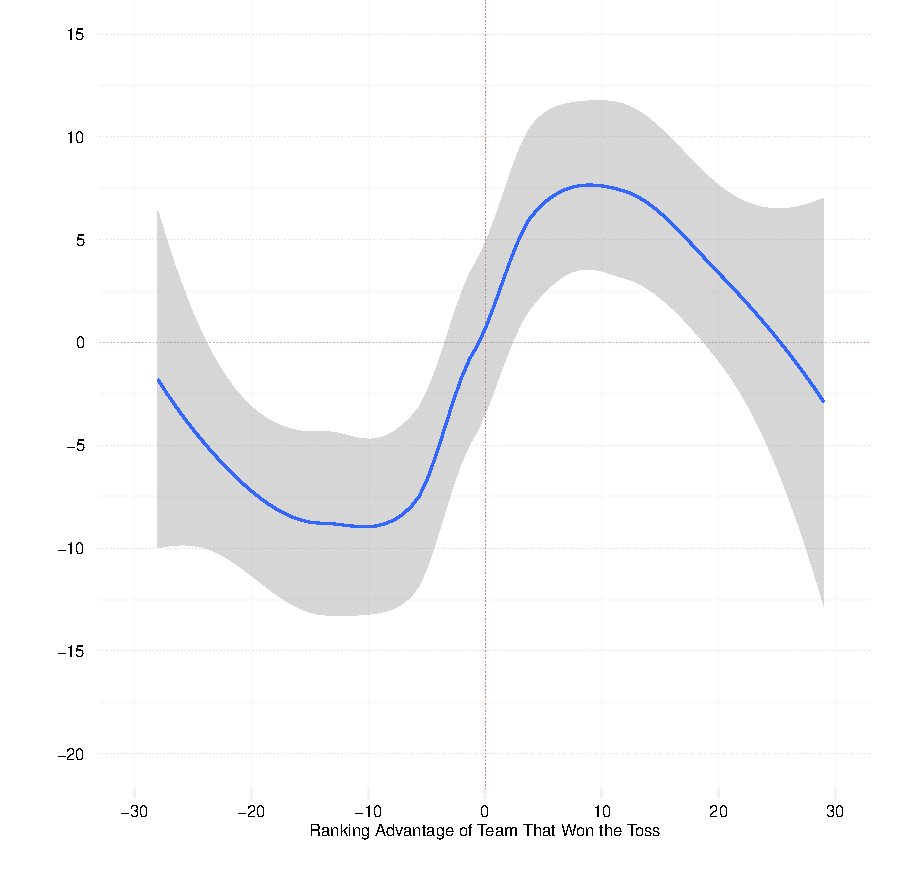
\includegraphics[scale=.85]{../figs/winbyRank.pdf}
\label{fig:ranks}
\end{figure}

This isn't a comprehensive inventory of analyses that one could do on the topic. But neither is it meant to be. There are some simple questions that still unanswered. For one, how does the toss advantage vary over time? Have teams become smarter? How the advantage vary by country -- are some countries better than others? Other more nuanced but commonly thought questions also remain. For one, students of the game suspect that the advantage of winning a toss in early English season is especially great. We propose to investigate these questions in a follow-up piece.

\clearpage
\bibliographystyle{apsr}
\bibliography{luckybib}

\end{document}